\chapter{Introduction}

The increase of computational power enabled the integration of deep learning concepts in real-world scenarios.
Training of large datasets for supervised learning models leads to a lot of problem solvers and automation in business and private areas of society.
The technology influences a large amount of people every day with rising tendency.
Well-known uses are algorithms for search, personalized adds, voice assistants, autonomous vehicles, transportation and network security.
\hfill \break
Scientist with technical knowledge integrade the concepts of deep learning into nearly every industry and branch.
Great examples for current real-world easements are in healthcare, marketing and agriculture:

IBM develops software that supports diagnosing, treating and predicting outcomes in medical situations.
Their deep learning algorithms have the ability to read and filter unstructured data, find similarities between patients and finding information in medical literature that helps to discover new insights.
Doctors benefit from personalized patient treatment plans and better analysis by the monitoring of patients. Researchers can discover new insights in drug development.
Currently the IBM Watson Healthcare software helps more than 230 healthcare organizations worldwide with more than 15,000 clients and partners. Their cognitive offerings have impacted care or social services for more than 295,000 people.
\cite{ibm-watson-healthcare, ibm-watson-facts}

Airbnb, an online marketplace for renting homes, uses deep neural networks for categorising its listing photos.
The decision of their customers is influenced by a diverse set of images.
Many home providers label their images wrong and have not enough variety in their collection.
Moreover, their total amount of photos is nearly half a billion images.
Deep learning helps them identifying the picture and presenting them on the site properly.
Moreover, they can detect certain objects in the images, which enable custom filters and searches for objects.
\cite{airbnb-ic-video, airbnb-ic-blog}

\begin{figure}[H]
    \centering
    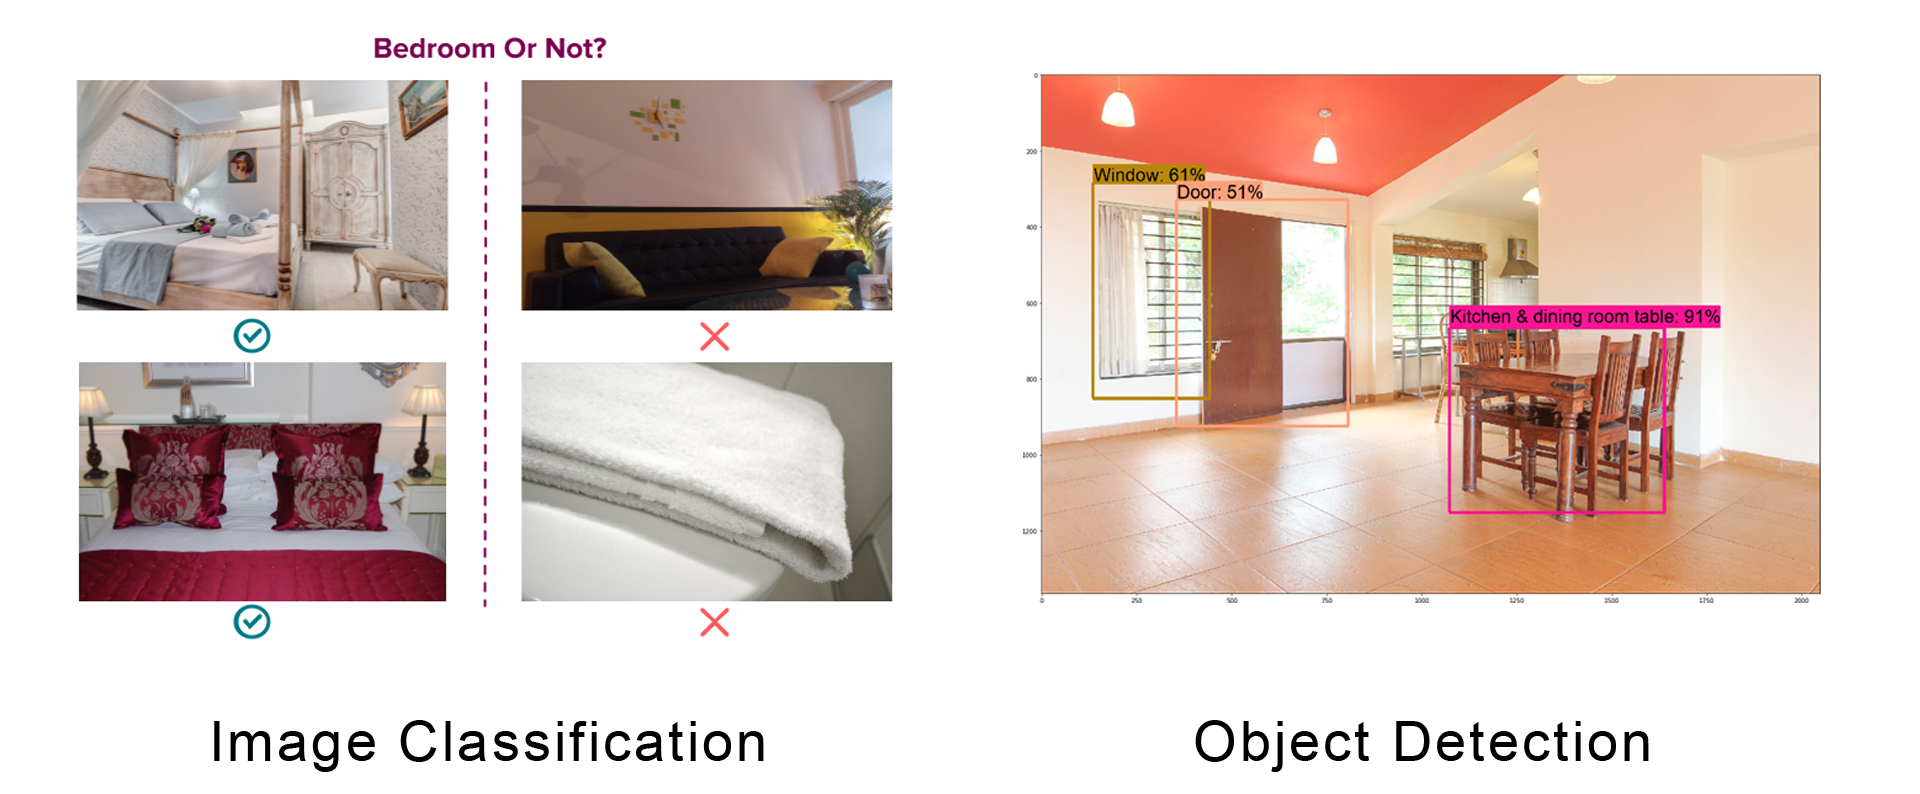
\includegraphics[width=\textwidth]{airbnb_classification_and_detection}
    \caption{\cite{airbnb_image_classification, airbnb_object_detection} Airbnb image classification and object detection}
    \label{fig:airbnb_image_classification}
\end{figure}

Connecterra developed an intelligent dairy farmer assistant.
They discovered that the production of milk is based on the animal’s health.
With an animal observation and machine learning they are able to diagnose problems early and provide health recommandations to the farmers.
\cite{tensorflow-stories, connecterra-video, connecterra-web}

The latest outstanding milestone in research: An AI algorithm developed by Google DeepMind had beaten two of the worlds's best StarCraft 2 players.
StarCraft, a Real-Time Strategy (RTS) game was called the "grand challenge" for AI because of the game complexity.
To win in this game the algorithm needs to develop continually new frontiers of strategic knowledge.
Moreover, there are crucial information hidden that must be actively discovered in real-time. On top of it there are a lot of units and buildings that must be controlled at once.
By winning against two of the world's best players without any game restrictions they mastered the biggest challenge in the most played mode.
It was achieved using a deep neural network that is trained by supervised learning and reinforcement learning.
The developed techniques could be useful in other problems which involve predictions over very long sequences such as weather predition and climate modeling.
\cite{alphastar}

These examples show that deep learning, a part of machine learning with the marketing reach of artificial intelligence, is more prensent than ever.
The media uses the terms "Artificial Intelligence (AI)", "Machine Learning (ML)" and "Deep Learning (DL)". They are all connected but not the same.
\hfill \break
Nvidia, an american technology company visualizes the relationship between these terms as concentric circles.
At first the largest term artificial intelligence was introduced.
After that was the emergence of machine learning and finally deep learning which fits inside both terms and drove major breakthroughs.
\cite{nvidia-ai-explained}

\begin{figure}[H]
    \centering
    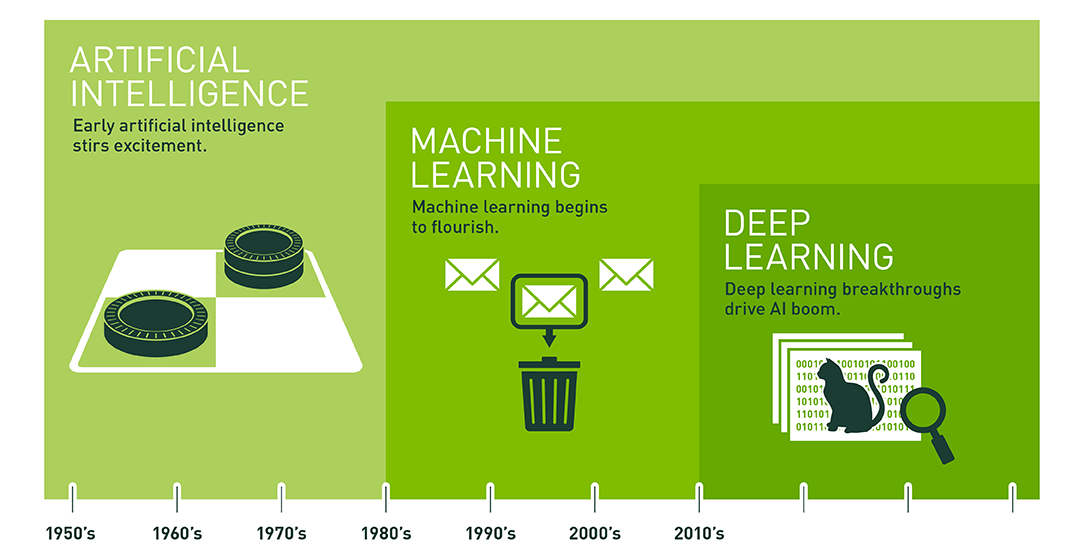
\includegraphics[width=\textwidth]{Deep_Learning_Icons_R5_PNG}
    \caption{\cite[page 5]{nvidia-ai-explained} Relationsship of AI, ML \& DL}
    \label{fig:ai_ml_dl_termns}
\end{figure}

Machine learning uses algorithms to parse data, learn from it and then make determinations or predictions.
In practice it is helping software to perform a result without the explicit programming of rules.
To be able to get answers from data using machine learning there are multiple steps involved:
\cite{nvidia-ai-explained, tensorflow-about}

\begin{figure}[H]
    \centering
    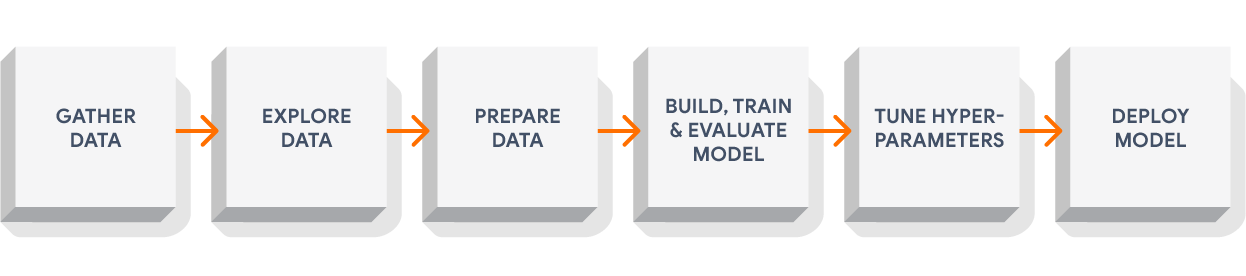
\includegraphics[width=\textwidth]{how_ml_works_tab2_graphic}
    \caption{\cite{tf_ml_steps_pipline} Steps to solving an machine learning problem}
    \label{fig:ml_steps_pipeline}
\end{figure}

In machine learning there are three main paradigms called supervised learning, unsupervised learning and reinforcement learning:

\begin{figure}[H]
    \centering
    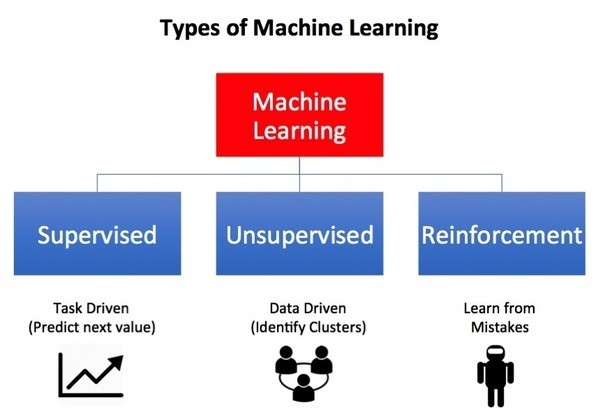
\includegraphics[width=\textwidth]{machine_learning_paradigms}
    \caption{\cite{ml_paradigms_image} Machine learning paradigms}
    \label{fig:ml_paradigms_image}
\end{figure}

In \textbf{supervised learning}, the network trains on a big dataset.
The dataset is composed of a lot of examples.
Each example has its correct result attached to it.
The examples are called features and their outcome is a label.
This approach is good for classification (categorial or discrete) and regression (numerical or continuous) problems.
\cite{nvidia_paradigms_blog}
\hfill \break
In contrast, \textbf{unsupervised learning} uses unlabelled data, because there is no desired outcome or correct answer.
The network tries to extract features and pattern on its own.
It can organize the data in different ways: clustering (separation of collections), anomaly detection, association
(feature correlation) and frequent pattern matching.
\cite{nvidia_paradigms_blog}
\hfill \break
In \textbf{reinforcement learning}, networks are agents and attempt to find the optimal way to accomplish a goal.
Agents are set on an environment, where the networks makes a decision.
An interpreter checks the decision and rewards or punishes the network.
This approach wants to find a long-term strategy and relies on learning from past feedback and exploration of new tactics.
\cite{nvidia_paradigms_blog}

Neural networks are inspired by the biology of a human brain.
A network consists of an input and output layer with at least one hidden layer.
Each layer is composed of nodes that are called neurons and connections between neurons which are called weights.
There are various differnet types of neural networks.
They differ based on their parameter representation and mathematical operations.
This article sticks with a classification of a deep neural network in a supervised learning manner.
The proposed technical approaches can be used with reinforcement learning as well.
Figure \ref{fig:dnn_3hidden_example} shows a fully connected deep neural network with one three layers:
\cite{nvidia-ai-explained, tensorflow-about}

\begin{figure}[H]
    \centering
    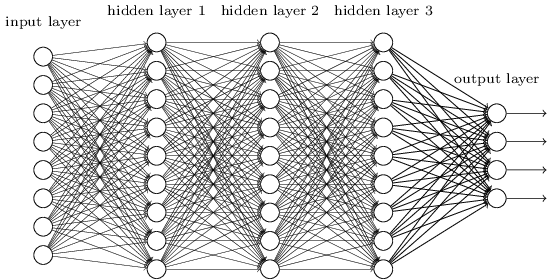
\includegraphics[scale=.6]{dnn_3hidden_example}
    \caption{\cite{dnn_3hidden_example_image} Example of a deep neural network}
    \label{fig:dnn_3hidden_example}
\end{figure}

To be abe to classify on data, the neural network has to be trained.
In the training phase "teaches" the network itself how to understand data by classifying records or making predictions. \cite{ibm-watson-healthcare}
The weights and neurons on each layer begin with random values which are improved over time to make the network more accurate.
In the training process a loss function quantifies how inaccurate the network is and a procedure called backpropagation is used to adjust each weight and neuron for an better accuracy.
\cite{nvidia-ai-explained, tensorflow-about}

\begin{figure}[H]
    \centering
    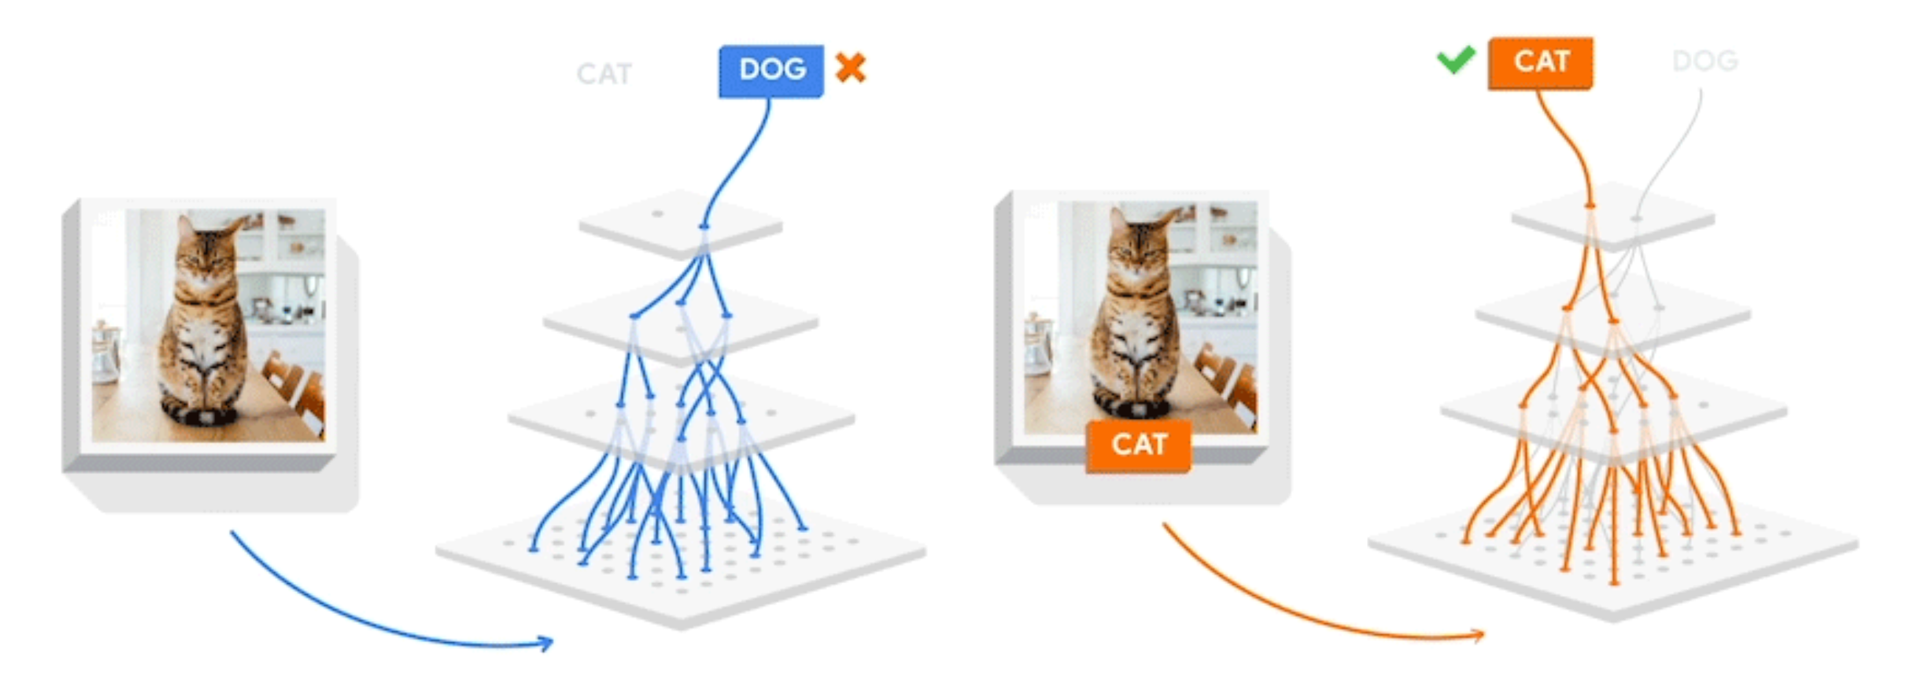
\includegraphics[width=\textwidth]{training-dnn-cat-example}
    \caption{\cite{tf_dnn_training_cat_example} Training of a neural network}
    \label{fig:tf_dnn_training_cat_example}
\end{figure}

The training result of a neural network is a model.
The model consists of all weight and neuron values.
\hfill \break
This model can predict all classifications it learned from the dataset.
A good representation for understanding the insight of a network is to take a closer look to the values each neuron stores.
Each neuron in the model learned an abstract representation of the data.
This results in a feature hierarchy between the different layers \cite{skymind_neural_network}.
Neurons on the first layers learn to detect lines from the input.
The layers after that learn combine the lines to shapes.
The last layers can recognize textures based on the shapes.
The textures together conclude to the final prediction.
Figure \ref{fig:tf_dnn_shapes_textures} shows a visual diagram of a network detecting lines, shapes, and textures:
\cite{nvidia-ai-explained, tensorflow-about}

\begin{figure}[H]
    \centering
    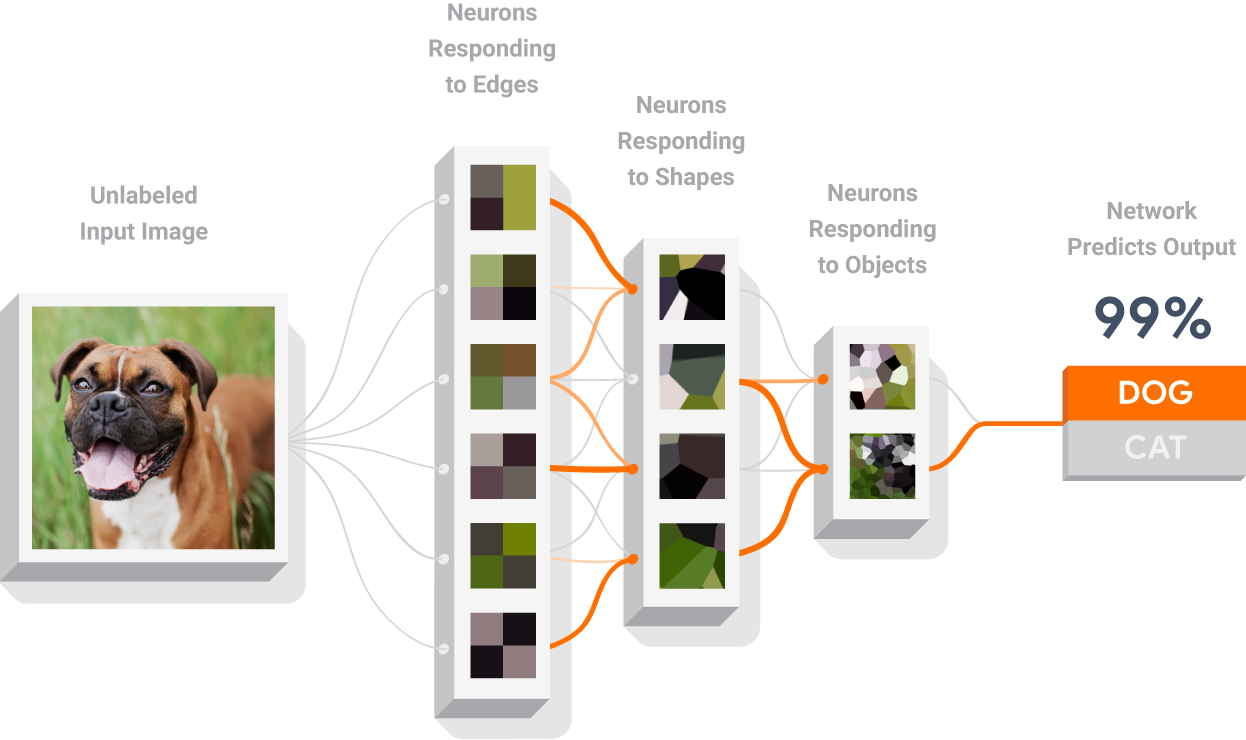
\includegraphics[width=\textwidth]{how_ml_works_tab3_graphic}
    \caption{\cite{tf_dnn_shapes_textures} Anatomy of a neural network}
    \label{fig:tf_dnn_shapes_textures}
\end{figure}

\section{Motivation}

These use-cases show great solutions for real-world problems solved with deep learning approaches.
However, current deep learning solutions are facing two major challenges:

AI is such a powerful tool that more and more people are concerned about misuses of the technology.
Many people claim a governance of AI by governments and social guidelines.
An open letter with the title "Research priorities for robust and beneficial artificial intelligence" by the Future of Life institute is currently signed by over 8,000 artificial intelligence experts, researchers and successful businessmen \cite{futureoflife-ai-open-letter, futureoflife-research-priorities}.
The letter affirms a great potential of artificial intelligence for society, but calls for concrete research on: "…how to reap its benefits while avoiding potential pitfalls" \cite{futureoflife-ai-open-letter}.
Furthermore the Future of Life institution presents 23 AI principles in the areas of research issues, ethics and values and longer-term issues. \cite{futureoflife-ai-principles}
\hfill \break
Another example is a white paper published by Google with the title "Perspectives on Issues in AI Governance".
Google which provides on of the biggest ecosystems for machine learning as an open source platform shares their point of view in explainability standards, fairness appraisal, safety considerations, human-AI collaboration and liability frameworks with commentaries on the issues and suggestions of actions \cite{google-ai-governance}.
Moreover, they invoke governments and civil society groups to contribute to the AI governance discussion.
According to Google there are already many regulations and legal codes that are broad enough to apply to AI and high level contentions by policymakers \cite[page 3]{google-ai-governance}.
Google acknowledges the first steps and hopes to help with their deeper insights for deeper discussions \cite[page 4]{google-ai-governance}.
\hfill \break
Besides the white paper they published their principles for using the technology.
They assess AI applications to be socially beneficial, avoiding unfair bias, built and tested for safety, are accountable to people, include privacy design principles, have high standards of scientific excellence and are made available for uses that concur with these principles.
In addition to their objectives for AI applications, they list areas where they will not design or deploy applications:
Technologies that cause harm, facilitate injury to people, violating internationally accepted norms or is against accepted principles of international law and human rights.
\cite{google-ai-principles}
\hfill \break
A similar approach has the German Telekom AG, one of the largest telecommunication providers in Europe.
In November 2018 they shared their guidelines for artificial intelligence in a public blog post.
They take actions under their guidelines of transparency, security, responsibility and caring for the customer.
\cite{telekom-ai-guidelines}
\hfill \break
These first discussions about AI ethics begun more frequently by technologists and policymakers, but the public opinion has not shaped much of these conversations today \cite{governanceai_public_report}.

The second obstacle is the ongoing improvement in machine learning:
\hfill \break
Deep learning techniques have been shining with a large number of labeled datasets and outperform many machine learning techniques.
With new attention to unsupervised and reinforement learning which are aiming to solve complex tasks without explicit knowledge improves the effort of creating datasets for training models \cite{continual-ai-blog, alphastar}.
However, most deep learning techniques are solving specific, isolated tasks which are not able to learn new tasks with a given model \cite{continual-ai-blog}.
Many real-world scenarios require the ability of multi-task learning.
Multi-task learning means that deep neural networks are able to learn multiple consecutive tasks without forgetting previous tasks \cite{elastic-weight-consolidation}.
This challenge results in the paradigm of "continual learning".
Other common designations are "incremental learning", "continuous learning" or "lifelong learning" \cite{lifelong-machine-learning-book, continual-ai-blog}.
The oldest term is "lifelong learning" and was used in areas outside of deep learning \cite{continual-ai-blog}.
This is why there were the introduction of modern terms like "continuous" or "continual", which are targeting specifically deep learning algorithms \cite{continual-ai-blog}.
The Oxford Dictionary says that "continuous" is five times more prominent than "continual" and refers to "no interruption" \cite{oxford-continual-continuous}. "Continual" on the other hand includes the meaning of "inbetween intervals" or "happening frequently" \cite{oxford-continual-continuous}.
The meaning of "Continual" is a closer definition to this article and will be used together with the term "incremental", which is a more technical for the domain.
\hfill \break
The goal of continual learning is such a challenge because of the "Catastrophic Forgetting" problem in deep neural networks.
Models forget information of previous tasks after being trained on a new task.
This occurs specifically because the weights in the network that are important for task A are updated to be able to predict task B correctly.
Current approaches typically ensure that the data from all tasks have to be available during training.
This means, every training will be a completely new model created, where forgetting does not occur because the optimization is joint by all tasks.
It is often called as a multitask learning paradigm.
\cite{incremental-moment-matching, continual-ai-blog}

\begin{figure}[H]
    \centering
    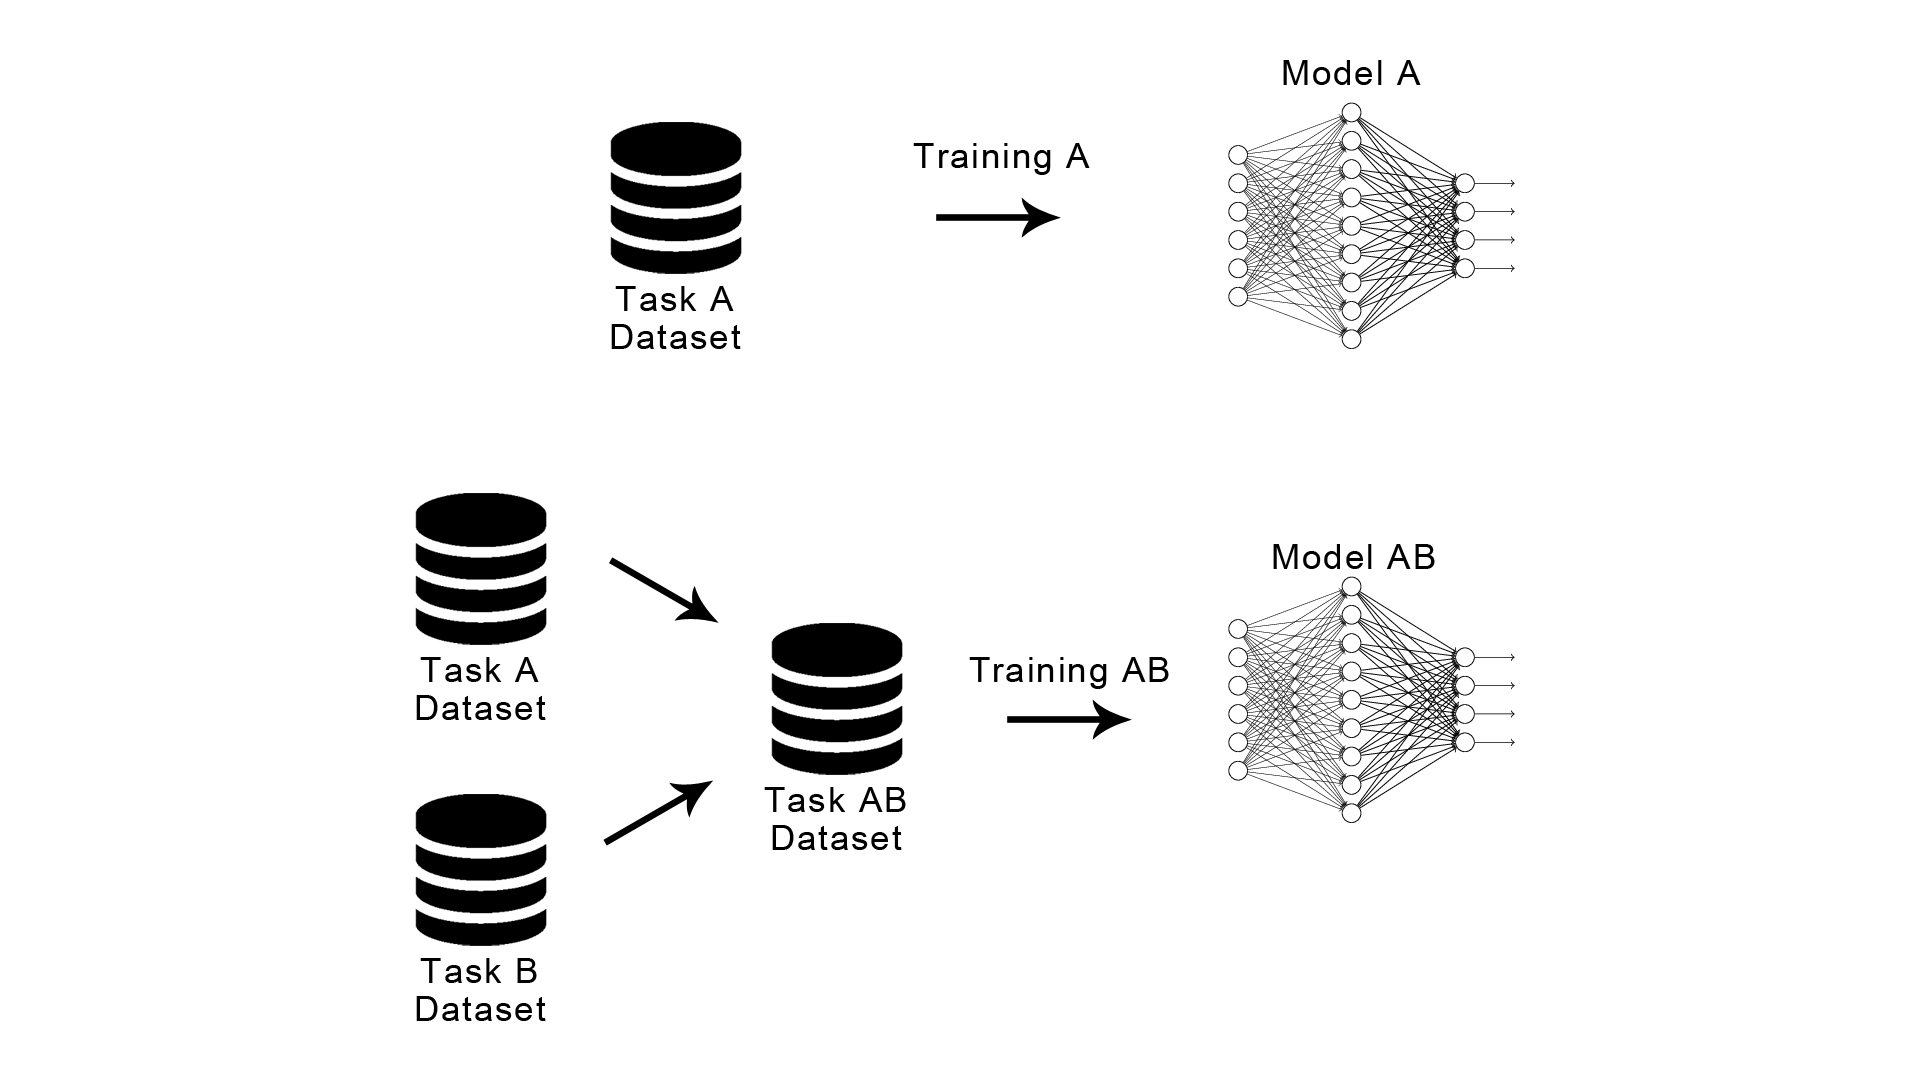
\includegraphics[width=\textwidth]{multitask_learning_paradigm}
    \caption{Multitask learning paradigm}
    \label{fig:intro_motivation_multitask_learning_paradigm}
\end{figure}

But this approach does not solve the problem properly and brings disadvantages along the way.
Continual learning wants to be adaptable and scalable.
Szenarios that keep changing over time are not covered by AI yet.
IT is hard to collect data for a representative dataset in time, even when the semantics keep chaning.
Current techniques will not be able to survive in these environments.
This is where continual learning really shines against current techniques.
Moreover, there is the term of scaling intelligence.
In large scaled models it is not possible to retrain the network for additional tasks because of a computation and time limit.
Or the integration of deep learning in edge devices limits the model on performance and memory.
In these cases it is not possible to store and extend the dataset as well as retraining the model in real-time.
The main idea behind continual learning is to process data once and than get rid of it.
This would enable a lightweight model that is able to adapt to any task.
These ideas of continuously and adaptively learning about new features would enable an autonomous incremental development and the ability of learning more complex skills and knowledge.
\cite{continual-ai-blog}

\begin{figure}[H]
    \centering
    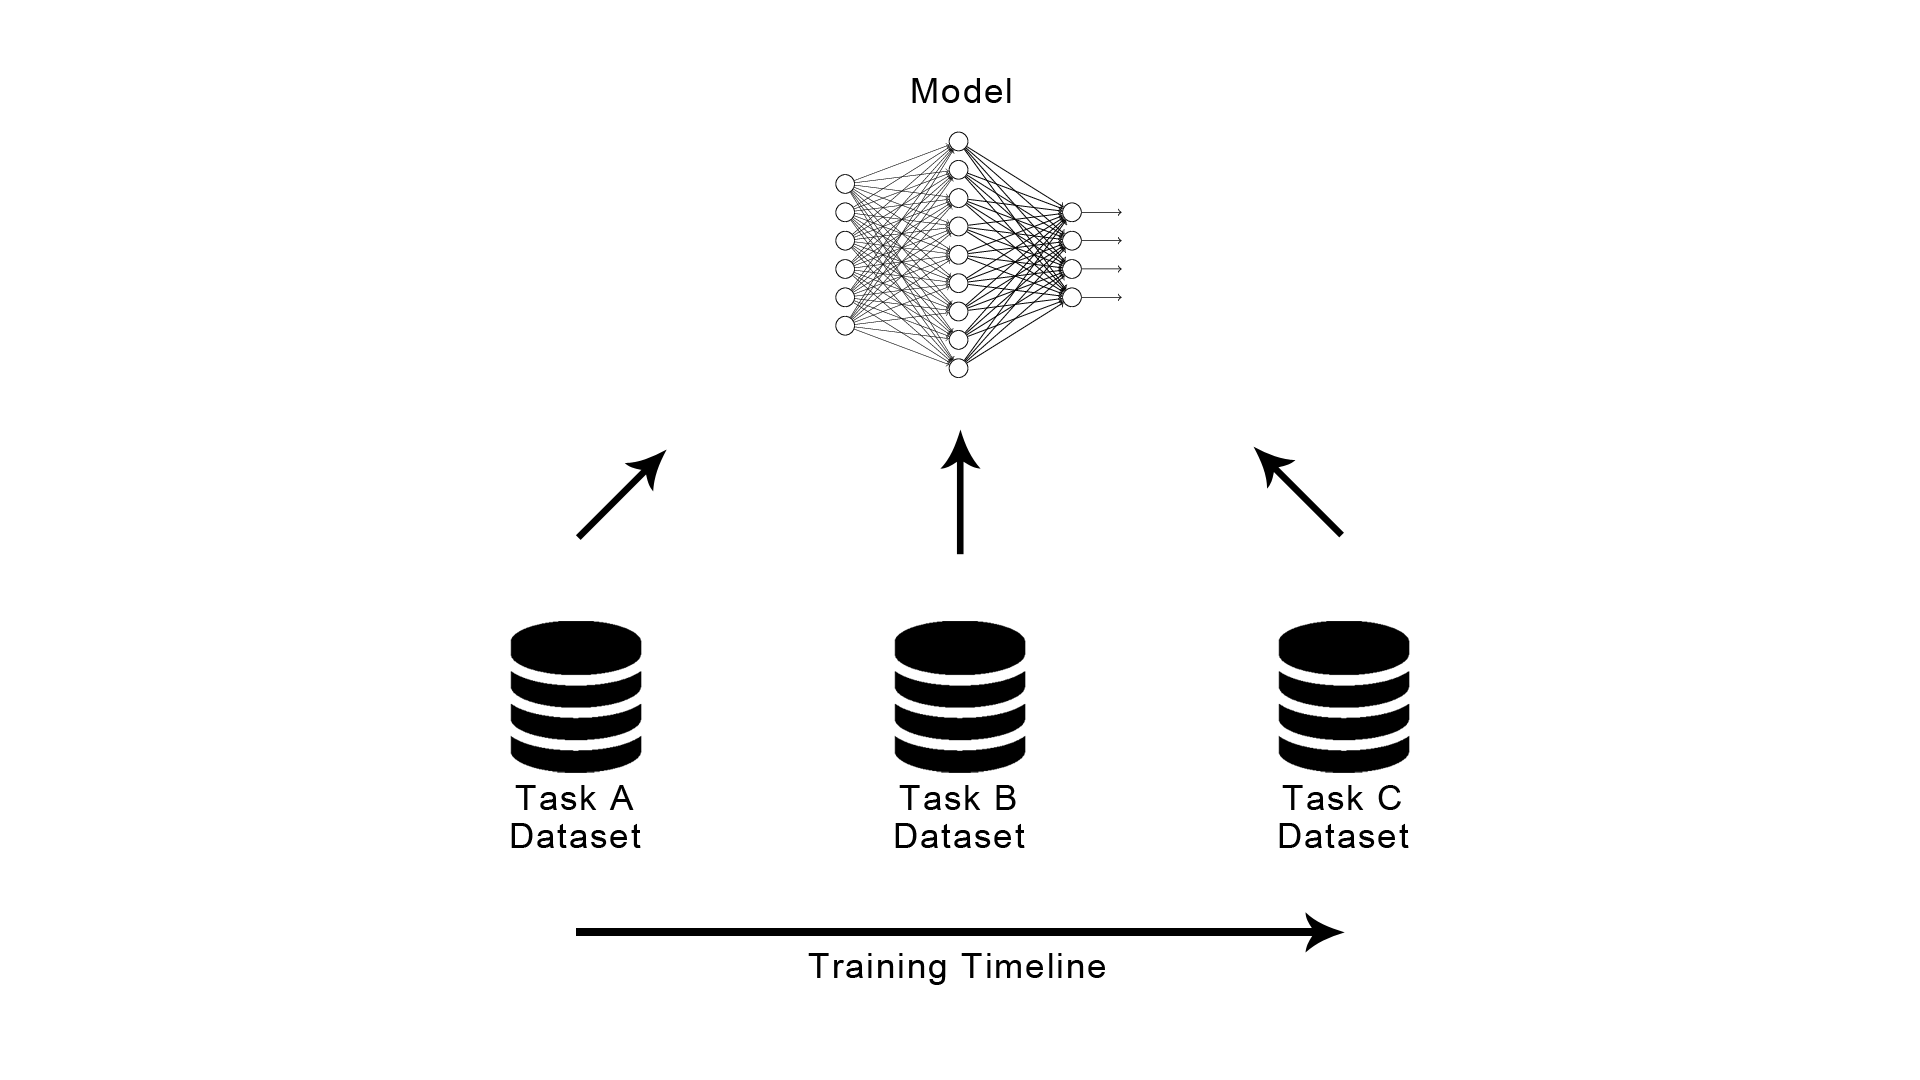
\includegraphics[width=\textwidth]{continual_learning_paradigm}
    \caption{Continual learning paradigm}
\end{figure}

Anatoly Gorshechnikov, CTO of Neurala Inc. presented great examples of use-cases that touch both challenges at the NVIDIA GTC Conference in 2017.
Neurala is a software company which offers consulting services to their clients.
Practical problems along the way are, that their clients do not like to share data.
Even when Neurala convinced their clients, that their data is needed to be able to build a meaningful model, the clients expect, that Neurala does not keep their data.
In the following months Neurala gets approached by some clients again, who asks them to integrate the new dataset to the previous.
Here comes the problem, that the dataset does not exist anymore.
\hfill \break
An even more extreme example he shares is a customer who is a toy manufacturer.
One requirement is that their toy recognizes other toys from the manufacturer.
The second demand is that the toy recognizes his owner.
Neurala solved the first requirement rather easy by a factory pretraining.
To solve the second demand, the model needs to be trained after the toy is sold.
One approach could be to record a video and transmit it to the cloud and retrain the network.
But because of ethical reasons there exist privacy laws that do not allow uploading images of kids or even related information to kids to the cloud.
So Neurala faced the challenge to add data on top of new data, without forgetting old data and without powerful servers and cloud access.
Moreover, the kids should be indentifies in seconds.
No one would use this feature, if they had to look at the toy for a long time.
\hfill \break
A great example, where current deep neural networks are not able to perform and the new paradigm of continual learning is needed.
\cite{neurala_video}

Moreover, continual learning is a key hurdle to be able to develop an artificial general intelligence.
This term thinks of a machine intelligence that is able to perform any intellectual task that a human being is able to.
For this scientific topic there are multiple non-profit organisations and companies like OpenAI, Google DeepMind and the AGI Society, who delve this topic existing.
Here is continual learning a major part that a model does not rely on a permanent existing dataset.

\section{Related Work}

As the time of writing exist mutiple approaches to overcome the problem of catastrophic forgetting.
The white paper "Continual Lifelong Learning with Neural Networks: A Review" \cite{lifelong_learning_review} summarises main challenges linked to lifelong learning and compares existing neural network approaches that alleviate catastrophic forgetting to different extends.
The book "Lifelong Machine Learning" \cite{lifelong-machine-learning-book} written by Zhiyuan Chen and Bing Liu coveres all of the important work in the field.
It explains all paradigms and current continual learning methods.
\newline
% elastic weight consolidation
One of the well-known approaches is the Elastic Weight Consolidation \cite{elastic-weight-consolidation}.
This technique tries to encourage all important parameters to stay close to the old task.
It proposes to add a term to the loss function that protects weights that are important for the previous sub-task(s) \cite{elastic-weight-consolidation}. 
Importance is determined by approximating the diagonal Fisher Information Matrix of the DNN \cite{cf_application_oriented_study, elastic-weight-consolidation}.
% better weight consolidation
An improvement to this approach shows the Better Weight Consolidation \cite{better-weight-consolidation}.
They specifically address the diagonal assumption made by the EWC algorithm \cite{better-weight-consolidation}.
Their presented solution is the computation of a rotation matrix for a more valid diagonal FIM assumption \cite{better-weight-consolidation}.
\newline
% Incremental Moment Matching
Incremental Moment Matching, another approach that trains ongoing sequential tasks on a new network and merges these two networks together by using the diagonal Fisher Information Matrix \cite{incremental-moment-matching}.
They propose two moment matching algorithms that are tested on various datasets \cite{incremental-moment-matching}.
\newline
% Natural Gradient Descent
The Natural Gradient Descent (NGD) proposes an approximation of the FIM for convolutional neural networks \cite{natural_gradient_descent}.
It consists of tracking a diagonal variance, not in parameter coordinates, but in a generalisation of the outer product \cite{natural_gradient_descent}.
They show that their matrix is a better approximation of the Fisher Information Matrix in several neural network architectures \cite{natural_gradient_descent}.
\newline
% iCaRL
iCaRL learns classifiers and a data representation simultaneously \cite{iCARL}.
It allows only the training data for a small number of classes to be present and new classes can be added progressively \cite{iCARL}.
The use of a convolutional neural network makes it incompatible with deep neural network architectures \cite{iCARL}.
The paper show with the experiments on CIFAR-100 and ImageNet ILSVRC 2012 that it can learn many classes incrementally over a long period of time \cite{iCARL}.
\newline
% DEN - Dynamically Expandable Networks
Dynamically Expandable Networks (DEN) propose a deep network architecture that learns a compact overlapping knowledge sharing structures among tasks \cite{DEN}.
It is done by performing a selective retraining which prevents semantic drift by splitting/duplicating units \cite{DEN}.
The algorithm was tested on multiple public datasets \cite{DEN}.
\newline
% LwF - Learning without Forgetting
% https://arxiv.org/abs/1606.09282
Learning without Forgetting (LwF) is a strategy in convolutional neural networks \cite{LwF}.
At first they lock the old fully connected layers \cite{LwF}.
They append new fully connected layers to the convolutional layers and train the new task \cite{LwF}.
After tat they integrate both knowledges by a joint training \cite{LwF}.
This framework is promising where both trainings are similar to each other \cite{incremental-moment-matching, LwF}.
\newline
% Keep and Learn
The authors of the paper "Keep and Learn: …" \cite{Keep_and_Learn} present several baseline models "…for preserving learned knowledge by modeling the high-level feature space and output space to be mutually informative, and constraining feature vectors to lie in the modeled space during training" \cite{Keep_and_Learn}.
In comparison to LwF and EWC, which are proposed for preventing multi-task learning, they focus on multi-center single-task learning \cite{Keep_and_Learn}.
This means the model is learned with a different data-chunk of the same task and access to each data-chunk restricted \cite{Keep_and_Learn}.
Multi-center single-task learning could be compared to an permuted datasets that are used in several other approaches \cite{Keep_and_Learn}.
They used it in the area of restricted data, where privacy issues set border to different data junks \cite{Keep_and_Learn}.
\newline
% FearNet
FearNet is a brain-inspired dual-memory system \cite{FearNet}.
Their memory consolidation is inspired by mechanisms occurring during sleep \cite{FearNet}.
It has two complementary memory centers, a short-term memory system that immediately learns new information for recent recall and a DNN for the storage of remote memories \cite{FearNet}.
FearNet also has a separate network that determines which memory center contains the associated memory required for prediction \cite{FearNet}.
It is tested on images and audio classification \cite{FearNet}.
\newline
% Selfless Sequential Learning
In contrast to parameter importance like EWC, Selfless Sequential Learning proposes a regularizer that encourages representation sparsity by means of neural inhibition \cite{Selfless_Sequential_Learning}.
This results in few active neurons and leaves free neurons for upcoming tasks \cite{Selfless_Sequential_Learning}.
Their regularizer only prevents other neurons in a local neighbourhood \cite{Selfless_Sequential_Learning}.
This method is inspired by the lateral inhibition processes in the brain \cite{Selfless_Sequential_Learning}.
\newline
% Synaptic Intelligence
Similar to EWC Synaptic Intelligence measure the importance of the tasks before \cite{Synaptic_Intelligence}.
But instead of using the Fisher Information Matrix, they are putting forward a method which computes an importance measure online and along the entire learning trajectory \cite{Synaptic_Intelligence}.
\newline
% several test studies
Several articles used these approaches and tested them on different models and multiple datasets with different circumstances.
They investigated if these solve catastrophic forgetting and can be deployed in in real-world scenarios.
Their outlines are that none of the approaches solve the problem completely.
\cite{measuring_cf_in_nns, cf_application_oriented_study}
\newline
The paper "Measuring Catastrophic Forgetting in Neural Networks" compares five different mechanisms (regularization, ensembling, rehearsal, dual-memory, and sparse-coding) on real-world images and sounds \cite{measuring_cf_in_nns}.
Their results are that the mechanism(s) vary on the training paradigm and type of data in the dataset \cite{measuring_cf_in_nns}.
But they conclude, that the catastrophic forgetting problem has yet to be solved \cite{measuring_cf_in_nns}.
\newline
"A comprehensive, application-oriented study of catastrophic forgetting in DNNS" \cite{cf_application_oriented_study} tests multiple methods on the most popular datasets \cite{cf_application_oriented_study}.
Their results are that there is no method that avoids Catastrophic Forgetting under application conditions \cite{cf_application_oriented_study}.

\section{Project Goals}
\label{project_goals}

This article deals with specific parts of previous works on overcoming catastrophic forgetting.
It takes a closer look into simplifying computation and interpretation of the Fisher Information Matrix used in different incremental learning methods with deep neural networks.
One of the algorithms is the Elastic Weight Consolidation.
As proposed later it uses the Fisher Information Matrix to protect weights of earlier learned tasks \cite{elastic-weight-consolidation}.
Their paper does not establish why they use the Fisher Information Matrix, in fact just the diagonal of this matrix.
So this article takes a closer look to an alternative computation.
Besides reimplementing the EWC algorithm and the expansion, show the performance of it on several sequential learning tasks (SLTs).

\subsection*{Dataset and construction of sequential learning tasks}

\begin{figure}[H]
    \centering
    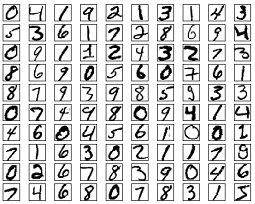
\includegraphics{mnist_100_digits}
    \caption{\cite{mnist_examples_image} MNIST dataset}
    \label{fig:intro_mnist_examples}
\end{figure}

This article uses the MNIST dataset for training the network and creating multiple tasks.
For the benchmarks MNIST is split into three types.
Each task of every type has its own separated train- and testsets.
All sequential learning tasks of the types used in this article have two subtasks.
The first task is $T_1$ and the second $T_2$.

\subsubsection*{Disjoint SLTs (D9-1 and D5-5)}

Two types are disjoint from the MNIST set.
MNIST is disjoint into each task five classes (D5-5 or nine classes for the first task and one class as second task (D9-1).

\subsubsection*{Permuted SLTs (P10-10)}

The thrid type consists of a permuted MNIST dataset.
The first task is the original mnist and the following tasks are permuted mnist sets.

% TODO why these benchmarks???
\iffalse

- since the paper shows poorly benchmarks parameters this article sticks with the best suited network for the mnist dataset
- moreover is relies on the application-oriented study, where a batch size of 100 with 2500 iteration together with the two disjoint and on permuted type and two tasks where used.

\fi